\documentclass[11pt,a4paper]{article}
\usepackage[utf8]{inputenc}
\usepackage[T1]{fontenc}
\usepackage[margin=2.3cm]{geometry}
\usepackage{amsmath,amssymb}
\usepackage{booktabs,array,tabularx,multirow}
\usepackage[table]{xcolor}
\usepackage{graphicx}
\usepackage{enumitem}
\usepackage{pgfplots}
\pgfplotsset{compat=1.17}
\usepackage{tikz}
\usetikzlibrary{arrows.meta,positioning,calc,shapes.geometric,fit}
\usepackage[most]{tcolorbox}
\usepackage[colorlinks=true,linkcolor=azul,urlcolor=azul]{hyperref}
\usepackage{fancyhdr}
\usepackage{titlesec}

\definecolor{azul}{HTML}{1F4E79}
\definecolor{azulc}{HTML}{E8F0F8}
\definecolor{verde}{HTML}{2E7D32}
\definecolor{verdec}{HTML}{E9F5EA}
\definecolor{naranja}{HTML}{C75B12}
\definecolor{naranjac}{HTML}{FDF1E6}
\definecolor{rojo}{HTML}{B3261E}
\definecolor{gris}{HTML}{666666}
\definecolor{grisc}{HTML}{F3F3F3}

\titleformat{\section}{\Large\bfseries\color{azul}}{\thesection}{0.6em}{}
\titleformat{\subsection}{\large\bfseries\color{azul}}{\thesubsection}{0.6em}{}
\setlist{itemsep=2pt,topsep=4pt}
\setlength{\parindent}{0pt}
\setlength{\parskip}{5pt}
\renewcommand{\arraystretch}{1.18}

\pagestyle{fancy}
\fancyhf{}
\fancyhead[L]{\small\color{gris}Guía de experimentos -- autoencoder recurrente de ciclos de marcha}
\fancyfoot[C]{\small\thepage}
\renewcommand{\headrulewidth}{0.3pt}

\newtcolorbox{intuicion}[1][Intuición]{colback=azulc,colframe=azul,fonttitle=\bfseries,title={#1},boxrule=0.6pt,arc=2pt,left=6pt,right=6pt,top=4pt,bottom=4pt,breakable}
\newtcolorbox{resultado}[1][Resultado]{colback=verdec,colframe=verde,fonttitle=\bfseries,title={#1},boxrule=0.6pt,arc=2pt,left=6pt,right=6pt,top=4pt,bottom=4pt,breakable}
\newtcolorbox{cuidado}[1][Cuidado]{colback=naranjac,colframe=naranja,fonttitle=\bfseries,title={#1},boxrule=0.6pt,arc=2pt,left=6pt,right=6pt,top=4pt,bottom=4pt,breakable}
\newtcolorbox{frase}{colback=grisc,colframe=gris,boxrule=0.4pt,arc=2pt,left=6pt,right=6pt,top=3pt,bottom=3pt,fontupper=\itshape,breakable}

\newcommand{\gr}{$^\circ$}
\newcommand{\mae}{\textsc{mae}}
\newcommand{\bpm}[2]{$\mathbf{#1}\boldsymbol{\pm}\mathbf{#2}$}

\title{\textbf{\color{azul}Guía de experimentos}\\[2pt]\large Autoencoder recurrente sobre ciclos de marcha:\\ qué se hizo, por qué, qué se logró y qué no}
\author{Documento de apoyo para la reunión de seguimiento}
\date{15 de octubre de 2026}

\renewcommand{\contentsname}{Índice}
\renewcommand{\abstractname}{Resumen}
\renewcommand{\figurename}{Figura}
\renewcommand{\tablename}{Tabla}
\begin{document}
\maketitle
\thispagestyle{fancy}

\begin{abstract}\noindent
Esta guía explica, con intuición y con números, todos los experimentos realizados sobre el autoencoder recurrente (GRU) del pipeline de la variedad de ciclos. Para cada experimento se responde: ¿qué problema atacaba?, ¿por qué se esperaba que funcionara?, ¿qué pasó?, ¿cómo se explica en una frase? Al final hay un guion para la reunión, preguntas probables y puntos que conviene confirmar. Los resultados negativos se incluyen con el mismo detalle que los positivos.
\end{abstract}

\setcounter{tocdepth}{1}
{\small\setlength{\parskip}{0pt}\tableofcontents}
\newpage

%=====================================================================
\section{El resumen en un minuto}

\begin{resultado}[Mensaje central]
El autoencoder GRU original tenía \textbf{dos defectos concretos}: (i) reconstruía con un error alto porque el decodificador ``olvidaba'' el código del ciclo a mitad del recorrido, y (ii) producía ciclos que \textbf{no cerraban} (el último punto no coincidía con el primero, unos 4.9\gr{} de diferencia). Se corrigieron ambos con dos cambios pequeños y se validaron con cinco semillas y prueba t pareada.
\end{resultado}

\begin{intuicion}[Qué son ``A'' y ``B'' (se usan en toda la guía)]
Son \textbf{la misma red}, un autoencoder recurrente (GRU) que en el cuaderno original se llama \texttt{rnn\_autoencoder}; solo cambia \emph{con qué se entrena}.
\textbf{A} se entrena con ciclos limpios y se le pide copiarlos (\emph{reconstruir}). \textbf{B} (la variante \emph{denoising}, \texttt{denoising\_rnn\_autoencoder}) se entrena con ciclos \emph{dañados} a propósito y se le pide devolver el ciclo limpio (\emph{corregir}).
\textbf{Los dos se evalúan con exactamente las mismas métricas} (sección \ref{sec:proto}); la tabla siguiente muestra solo las que más se mueven en cada caso. De dónde salen y cómo se llaman en el cuaderno: sección \ref{sec:modelos}.
\end{intuicion}

\begin{center}
\begin{tabular}{lccc}
\toprule
 & \textbf{Original} & \textbf{Mejorado (1 mod.)} & \textbf{Ensamble de 5} \\
\midrule
Modelo A: error \mae{} & 5.17\gr & 4.11\gr & \textbf{3.91\gr} \\
Modelo A: salto de cierre & 4.94\gr & 0.87\gr & \textbf{0.55\gr} \\[3pt]
Modelo B: error \mae{} & 5.35\gr & 4.83\gr & \textbf{4.74\gr} \\
Modelo B: salto de cierre & 3.45\gr & 0.57\gr & \textbf{0.36\gr} \\
Modelo B: ganancia de corrección & 0.280 & 0.337 & \textbf{0.349} \\
\bottomrule
\end{tabular}
\end{center}
{\small ``Original'': cifras del cuaderno inicial. ``Mejorado'': promedio de 5 semillas del modelo con los cambios propuestos. La ganancia de corrección de A no aparece porque no fue el objetivo del cambio probado en A: con cinco semillas pasó de 0.208 (original reproducido) a 0.189 (mejorado; $p=0.077$), es decir, no mejoró; el ensamble de A tiene 0.229. En negrilla, la mejor cifra de cada fila. Detalles y salvedades en las secciones \ref{sec:escalera} y \ref{sec:limites}.}

\textbf{Cuatro ideas para llevarse:}
\begin{enumerate}
\item \textbf{Dos cambios explican casi toda la mejora}: repetir el código del ciclo en cada paso del decodificador (menos error) y penalizar que el ciclo no cierre (menos salto). Ambos son pequeños y baratos.
\item \textbf{Hay dos modelos con dos trabajos distintos}: A (entrenado con ciclos limpios) reconstruye con fidelidad; B (entrenado con ciclos dañados) corrige trayectorias raras. No son intercambiables ni se mezclan bien (veredicto completo en la sección \ref{sec:veredicto}).
\item \textbf{La mayoría de las ideas adicionales no mejoraron} (suavidad, atención, características extra, etc.). Eso también es un resultado: delimita dónde está el cuello de botella.
\item \textbf{Aún no se alcanza el error de PCA} (2.78\gr) en fidelidad, pero PCA no sirve para corregir. Y B mejorado (0.34--0.35) sigue por debajo del autoencoder convolucional denoising del cuaderno original (0.41) en corrección (ver sección \ref{sec:ab}).
\end{enumerate}

%=====================================================================
\section{Veredicto: qué modelo es mejor y cuánto mejoró}
\label{sec:veredicto}

\begin{resultado}[Respuesta directa]
Entre los dos modelos recurrentes, \textbf{el modelo A mejorado es el mejor para reconstruir} y \textbf{el modelo B mejorado es el mejor para corregir}; ninguno gana en todo, y ambos mejoraron frente a su versión original en todas las métricas que se les midieron.

El \textbf{modelo A} (entrenado con ciclos limpios), en ensamble de 5, alcanzó un \mae{} de \textbf{3.91\gr} (el original tenía 5.17\gr: una mejora de \textbf{24\%}) y un salto de cierre de \textbf{0.55\gr} (el original, 4.94\gr: una mejora de \textbf{89\%}). Como modelo individual (promedio de 5 semillas) obtuvo \mae{} $4.11\pm0.05$\gr{} ($-20\%$) y salto $0.87\pm0.11$\gr{} ($-82\%$).

El \textbf{modelo B} (entrenado con ciclos dañados), en ensamble de 5, alcanzó una ganancia de corrección de \textbf{0.349} (el original tenía 0.280: \textbf{$+25\%$}), con un \mae{} de \textbf{4.74\gr} (original 5.35\gr: $-11\%$) y un salto de cierre de \textbf{0.36\gr} (original 3.45\gr: $-90\%$). Como modelo individual obtuvo corrección $0.337\pm0.007$ ($+20\%$), \mae{} $4.83\pm0.07$\gr{} ($-10\%$) y salto $0.57\pm0.05$\gr{} ($-84\%$).
\end{resultado}

\textbf{Cuál elegir.} Si se debe elegir un solo modelo, depende del objetivo: A si importa reproducir el ciclo con el menor error (3.91\gr{} frente a 4.74\gr{} de B), y B si importa devolver una versión típica a partir de un ciclo atípico (corrección 0.349 frente a 0.229 de A en ensamble). B, además, cierra mejor el ciclo (0.36\gr{} frente a 0.55\gr).

\begin{center}
\footnotesize
\setlength{\tabcolsep}{4pt}
\begin{tabular}{llcc}
\toprule
\textbf{Objetivo} & \textbf{Mejor} & \textbf{Ensamble de 5 (1 modelo)} & \textbf{Rival: ensamble (1 modelo)} \\
\midrule
Reconstruir con fidelidad (\mae{}) & \textbf{A} & \textbf{3.91\gr} (4.11\gr) & B: 4.74\gr{} (4.83\gr) \\
Cerrar el ciclo (salto) & \textbf{B} & \textbf{0.36\gr} (0.57\gr) & A: 0.55\gr{} (0.87\gr) \\
Corregir ciclos dañados (ganancia) & \textbf{B} & \textbf{0.349} (0.337) & A: 0.229 \\
\bottomrule
\end{tabular}
\end{center}
{\small Convención de negrillas: en todas las tablas numéricas de este documento la negrilla marca la cifra relevante, es decir, la mejor de la comparación o la que se cita en el texto.}

\begin{cuidado}[Salvedades del veredicto]
\begin{itemize}
\item \textbf{PCA sigue siendo mejor en fidelidad} (\mae{} 2.78\gr), y \textbf{el autoencoder convolucional denoising del cuaderno original sigue siendo mejor corrigiendo} (0.412 frente a 0.349 de B en ensamble). Este último no se reevaluó con cinco semillas.
\item Las cifras de ``ensamble'' vienen de un único ensamble por configuración (incertidumbre no medida); las de ``1 modelo'' son el promedio de 5 semillas y son las validadas con prueba t.
\item Contra la reproducción propia del modelo original con el mismo protocolo, las mejoras de \mae{} son menores: $-18\%$ en A (4.99 $\to$ 4.11) y $-8\%$ en B (5.25 $\to$ 4.83).
\item A \textbf{no} mejoró su ganancia de corrección: 0.208 (original reproducido) frente a 0.189 (mejorado), $p=0.077$ con cinco semillas, y 0.229 en el ensamble. Su ganancia de tipicidad bajó algo ($0.345\to0.326$, $p=0.034$). La cifra 0.152 del cuaderno original difiere de la reproducida y no se identificó la causa.
\item Los hiperparámetros se eligieron mirando el conjunto de control y la evaluación III no se recalculó para los modelos mejorados: las cifras son algo optimistas.
\end{itemize}
\end{cuidado}

\subsection*{Entonces, ¿por qué no usar PCA ni el autoencoder convolucional denoising?}

Con las cifras actuales \textbf{no hay una razón basada en métricas para preferir la RNN} sobre PCA en fidelidad, ni sobre el autoencoder convolucional denoising en corrección. La tabla pone todo junto (la RNN en su versión mejorada y en ensamble; los demás, tal como están en el cuaderno original).

\begin{center}
\small
\begin{tabular}{lccc}
\toprule
 & \textbf{\mae{} (\gr)} & \textbf{Salto (\gr)} & \textbf{Corrección} \\
\midrule
PCA & \textbf{2.78} & 3.41 & 0.207 \\
Proceso gaussiano periódico & 3.30 & 0.60 & 0.215 \\
Autoencoder convolucional denoising & 4.07 & 1.88 & \textbf{0.412} \\
Modelo A mejorado (ensamble) & 3.91 & 0.55 & 0.229 \\
Modelo B mejorado (ensamble) & 4.74 & \textbf{0.36} & 0.349 \\
\bottomrule
\end{tabular}
\end{center}
{\small Negrilla: mejor valor de la columna. Las filas de la RNN son un único ensamble; las demás, una sola corrida del cuaderno.}

\begin{cuidado}[Lectura honesta]
\begin{itemize}
\item \textbf{Fidelidad:} PCA (2.78\gr) y hasta el proceso gaussiano periódico (3.30\gr) reconstruyen mejor que cualquier RNN.
\item \textbf{Corrección:} el convolucional denoising (0.412) corrige mejor que B (0.337 con un modelo, 0.349 en ensamble).
\item \textbf{Cierre del ciclo:} es lo único donde la RNN mejorada queda al frente (B en ensamble, 0.36\gr), y solo por poco frente al proceso gaussiano (0.60\gr); un solo modelo A (0.87\gr) no lo supera.
\item \textbf{La comparación favorece a la RNN:} sus hiperparámetros se afinaron mirando el conjunto de control; los de PCA y del convolucional no, y sus cifras son de una sola corrida. Aun así, la RNN no los supera.
\end{itemize}
\end{cuidado}

\textbf{Razones posibles para seguir con la RNN (ninguna medida aquí):} que el proyecto la haya definido como el modelo a mejorar, o que la aplicación (exoesqueleto) necesite algo que PCA no da, como dinámica en el tiempo o ciclos de distinta longitud. Conviene confirmarlo con el tutor.

\textbf{Qué se propone:}
\begin{enumerate}
\item Plantear la pregunta de fondo: ¿se mejora la RNN por decisión de diseño, o se busca el mejor modelo? Si es lo segundo, hoy la respuesta es PCA para fidelidad y el convolucional denoising para corrección.
\item Aplicar al convolucional denoising las mismas mejoras que funcionaron (pérdida de cierre y, si cabe, repetir el código). No está probado, pero es el experimento más informativo.
\item Reevaluar PCA y el convolucional con las mismas cinco semillas y el mismo protocolo, para una comparación justa.
\end{enumerate}

%=====================================================================
\section{Vocabulario con intuición}

\begin{tabularx}{\textwidth}{>{\bfseries\raggedright\arraybackslash}p{3.1cm}>{\raggedright\arraybackslash}X}
\toprule
Término & Intuición \\
\midrule
Ciclo de marcha & Una zancada completa, remuestreada a 101 puntos (de 0\% a 100\% del ciclo) para seis ángulos: cadera, rodilla y tobillo, izquierda y derecha. Es una ``tarjeta'' de $101\times 6$ números. \\
Autoencoder & Una máquina que comprime la tarjeta en un código corto y luego intenta reconstruirla. Es como describir una canción en una frase y pedirle a otra persona que la tararee a partir de la frase. \\
Vector latente $z$ & El código corto (16 o 32 números). Es la ``frase'' que resume el ciclo. \\
GRU & Un tipo de red recurrente: lee la secuencia paso a paso y mantiene una memoria que se va actualizando. \\
Codificador / decodificador & El primero lee el ciclo y produce $z$. El segundo recibe $z$ y dibuja el ciclo punto a punto. \\
\mae{} (error absoluto medio) & Cuántos grados se equivoca la reconstrucción en promedio, en cada punto y ángulo. Menor es mejor. \\
Salto de cierre (\emph{endpoint jump}) & Diferencia entre el punto 0\% y el punto 100\% del ciclo reconstruido. Un ciclo real es periódico: debería cerrar, es decir, el salto debería ser $\approx 0$. \\
Denoising & Entrenar con ciclos \emph{dañados} a propósito (más amplitud, desplazados, con ruido, corridos en fase) pidiendo que la salida sea el ciclo \emph{limpio}. Enseña a ``arreglar'' trayectorias raras. \\
Ganancia de corrección & Qué fracción del daño se logra deshacer: $1-\mae(\text{corregido},\text{limpio})/\mae(\text{dañado},\text{limpio})$. 0 es no arreglar nada; 1 es arreglarlo todo. \\
Modelo A / modelo B & Misma red (autoencoder GRU). A se entrena con ciclos limpios; B con ciclos dañados (denoising). Ver sección \ref{sec:modelos}. \\
Original / mejorado & ``Original'': el modelo tal como está en el cuaderno inicial (o reentrenado igual, ``reproducido''). ``Mejorado'': con el código en cada paso y la pérdida de cierre. \\
Semilla & El número que fija el azar inicial (pesos y orden de los datos). Dos entrenamientos con distinta semilla dan resultados algo distintos. \\
Ensamble & Entrenar 5 modelos con semillas distintas y promediar sus salidas. El azar de cada uno se cancela parcialmente. \\
Prueba t pareada & Compara dos variantes semilla a semilla. Si la mejora aparece en todas las semillas con poca dispersión, el valor $p$ es pequeño. \\
\bottomrule
\end{tabularx}

%=====================================================================
\section{De dónde vienen los modelos y cómo se llaman}
\label{sec:modelos}

Todo el trabajo parte de un cuaderno del pipeline original que compara siete modelos sobre los mismos datos. Esta sección fija los nombres para no confundirse más adelante.

\begin{intuicion}[Dónde está el cuaderno de origen]
\raggedright
\begin{itemize}
\item \textbf{Cuaderno:} \texttt{10\_cycle\_manifold\_models.ipynb}\\
\textbf{Ruta:} \texttt{NeuroStrideAI/01-experimentation/notebooks/} (en el ZIP compartido: \texttt{NeuroStrideAI (4)/NeuroStrideAI/01-experimentation/notebooks/}).
\item \textbf{Datos de entrada} (los ciclos de 101 puntos y la partición por sujeto): los genera \texttt{09\_cycle\_manifold\_data\_preparation.ipynb} en \texttt{01-experimentation/data/derivatives/cycle\_manifold/} (archivo \texttt{cycles\_normalized.parquet}).
\item \textbf{Resultados de ese cuaderno} (las cifras ``originales'' de esta guía): \texttt{01-experimentation/outputs/cycle\_manifold\_models/}, con \texttt{control\_fidelity\_metrics.csv}, \texttt{synthetic\_correction\_metrics.csv}, \texttt{case\_typicality\_metrics.csv} y el resumen \texttt{model\_evaluation\_summary.csv}.
\item \textbf{Cuadernos vecinos:} el 12 (\texttt{12\_phase\_normative\_gp\_models.ipynb}) aporta el kernel periódico del proceso gaussiano; el 11 (grafo de articulaciones) no se usó en esta guía.
\end{itemize}
\end{intuicion}

Dentro del cuaderno 10, cada modelo aparece con un nombre de código. Esta es la traducción:

\begin{center}
\small
\begin{tabularx}{\textwidth}{@{}>{\ttfamily\raggedright\arraybackslash}p{4.4cm}>{\raggedright\arraybackslash}p{3.5cm}>{\raggedright\arraybackslash}X@{}}
\toprule
\textnormal{\textbf{Nombre en el cuaderno}} & \textbf{Nombre en esta guía} & \textbf{Qué es (sección del cuaderno)} \\
\midrule
control\_mean & Media de controles & Promedio de los ciclos de entrenamiento en cada fase (2) \\
pca & PCA & Proyección lineal a pocas componentes (2) \\
autoencoder\_1d & Autoencoder convolucional & Autoencoder con convoluciones 1D (3) \\
denoising\_autoencoder\_1d & Autoencoder convolucional denoising & El anterior, entrenado con ciclos dañados (3) \\
\textbf{rnn\_autoencoder} & \textbf{Modelo A} & \textbf{Autoencoder recurrente (GRU) entrenado con ciclos limpios (3b)} \\
\textbf{denoising\_rnn\_autoencoder} & \textbf{Modelo B} & \textbf{La misma GRU entrenada con ciclos dañados (3b)} \\
gp\_periodic\_residual & Proceso gaussiano periódico & Media de controles más un residuo modelado con un proceso gaussiano de kernel periódico (3c) \\
\bottomrule
\end{tabularx}
\end{center}

\textbf{Por qué esta guía se centra en A y B.} Eran los dos modelos con mayor error de reconstrucción entre los que aprenden de los datos (5.17\gr{} y 5.35\gr{}; la media de controles, que no aprende nada, tiene 8.77\gr{}) y los que se quiso mejorar. El resto (PCA, proceso gaussiano, autoencoders convolucionales) se usa solo como referencia.

\textbf{Qué quieren decir las etiquetas.}
\begin{itemize}
\item \textbf{A y B} no son dos arquitecturas distintas: ambos son la GRU del cuaderno. A recibe ciclos limpios y debe devolverlos; B recibe ciclos dañados (más amplitud, desplazamiento vertical, ruido y corrimiento de fase) y debe devolver el ciclo limpio.
\item \textbf{Original} = tal como está en el cuaderno (cifras 5.17 y 5.35) o reentrenado con el mismo protocolo (``reproducido'': 4.99 y 5.25). \textbf{Mejorado} = original más los dos cambios propuestos (código en cada paso y pérdida de cierre); para A, además, latente de 32 y $w=0.1$. \textbf{Ensamble} = promedio de las salidas de 5 modelos con semillas distintas.
\end{itemize}

%=====================================================================
\section{El punto de partida}

Estas son las cifras que el cuaderno 10 reporta para los siete modelos (columnas del archivo \texttt{model\_evaluation\_summary.csv}). \textbf{Todos los modelos se miden con las mismas métricas}; cada columna se explica en la sección \ref{sec:proto}.

\begin{center}
\footnotesize
\setlength{\tabcolsep}{4pt}
\begin{tabular}{lccccc}
\toprule
 & \textbf{\mae{}} & \textbf{Salto} & \textbf{Ganancia de} & \textbf{Ganancia de} & \textbf{Intervención} \\
 & \textbf{(\gr)} & \textbf{(\gr)} & \textbf{corrección} & \textbf{tipicidad} & \textbf{(\gr)} \\
\midrule
Media de controles & 8.77 & \textbf{0.60} & $-0.121$ & 0.132 & 10.83 \\
PCA & \textbf{2.78} & 3.41 & 0.207 & 0.127 & 3.86 \\
Autoencoder convolucional & 3.30 & 3.11 & 0.252 & 0.182 & 4.83 \\
Autoencoder convolucional denoising & 4.07 & 1.88 & \textbf{0.412} & 0.376 & 5.98 \\
Proceso gaussiano periódico & 3.30 & \textbf{0.60} & 0.215 & 0.192 & 3.86 \\
\rowcolor{naranjac}\textbf{Modelo A} (RNN) & 5.17 & 4.94 & 0.152 & 0.349 & 8.12 \\
\rowcolor{naranjac}\textbf{Modelo B} (RNN denoising) & 5.35 & 3.45 & 0.280 & \textbf{0.385} & 7.89 \\
\bottomrule
\end{tabular}
\end{center}

{\small Negrilla: mejor valor de la columna (la intervención no tiene ``mejor''). Fondo naranja: modelos A y B. La media de controles tiene el salto más bajo de forma trivial: su salida es un promedio de ciclos.}

\textbf{Cómo leer la tabla.} \mae{} y salto miden \emph{fidelidad} (evaluación I); la ganancia de corrección mide qué tanto se deshace un daño artificial (evaluación II); la ganancia de tipicidad y la intervención se miden sobre casos externos (evaluación III). A y B tienen las cinco columnas: A tiene 0.152 de corrección y B 0.280. Lo que los distingue no es qué métricas se les aplican, sino \emph{en cuáles destacan} por la forma en que se entrenaron.

\textbf{Qué se observa.} Entre los modelos que aprenden de los datos, A y B tienen el mayor error (5.17\gr{} y 5.35\gr{}) y los mayores saltos de cierre (4.94\gr{} y 3.45\gr{}, frente a 3.41\gr{} de PCA). La media de controles no aprende nada; por eso su error (8.77\gr{}) no cuenta como referencia de modelo. B tiene la mayor ganancia de tipicidad (0.385), pero el autoencoder convolucional denoising tiene la mayor ganancia de corrección (0.412).

\begin{intuicion}[Por qué A y B eran el eslabón débil en fidelidad]
Al revisar la arquitectura aparecieron dos causas probables, y cada una sugiere una reparación:
\begin{itemize}
\item \textbf{Olvido.} El código $z$ solo entraba al decodificador como estado inicial. Al ir dibujando los 101 puntos, la memoria se diluye: es como dictarle una dirección a alguien una sola vez y esperar que la recuerde después de 100 pasos.
\item \textbf{Nadie pedía cerrar el ciclo.} La función de pérdida solo mide el error punto a punto. Si el último punto queda lejos del primero, no hay castigo específico. Un ciclo de marcha, en cambio, es una curva \emph{cerrada}.
\end{itemize}
\end{intuicion}

%=====================================================================
\section{Cómo se midió}
\label{sec:proto}

\begin{itemize}
\item \textbf{Datos.} 461 ciclos válidos de 64 personas (video, AlphaPose a 30 fps). Partición \emph{por sujeto} para evitar fuga de información: entrenamiento 240 ciclos / 28 sujetos de control; validación 44 / 6; \emph{control\_test} 47 / 7; \emph{case\_external\_test} 130 / 23. Cada ángulo se estandariza con estadísticas del entrenamiento.
\item \textbf{Entrenamiento.} Optimizador adaptativo (Adam), tasa 1e-3, lote 64, hasta 100 épocas, parada temprana con paciencia 12 sobre validación, recorte de gradiente 1.0, 48 unidades ocultas. La pérdida de entrenamiento es el error cuadrático medio sobre los ángulos estandarizados (más, en las versiones mejoradas, el término de cierre); el \mae{} en grados es la métrica de evaluación, no la pérdida.
\item \textbf{Tres evaluaciones, las mismas para todos los modelos} (tabla siguiente).
\item \textbf{Cinco semillas} (42, 1, 7, 123, 2024) y prueba t pareada para toda mejora que se quiera afirmar. Una sola semilla se usó solo para explorar.
\end{itemize}


\begin{center}
\footnotesize
\begin{tabularx}{\textwidth}{@{}>{\raggedright\arraybackslash}p{2.2cm}>{\raggedright\arraybackslash}p{3.0cm}>{\raggedright\arraybackslash}p{2.8cm}>{\raggedright\arraybackslash}X@{}}
\toprule
\textbf{Evaluación} & \textbf{Qué se le da al modelo} & \textbf{Métrica} & \textbf{Cómo se lee} \\
\midrule
\textbf{I. Fidelidad} (reconstrucción) & 47 ciclos limpios de control no vistos (\emph{control\_test}) & \mae{} (\gr) & Error medio punto a punto entre salida y ciclo original. Menor es mejor. \\
 & & RMSE (\gr) & Igual, pero castiga más los errores grandes. Menor es mejor. \\
 & & Salto de cierre (\gr) & $|$salida(0\%) $-$ salida(100\%)$|$. Un ciclo periódico cierra; menor es mejor. \\
\midrule
\textbf{II. Corrección} & Los mismos 47 ciclos, \emph{dañados} artificialmente (misma receta que usa B al entrenar) & Ganancia de corrección & $1-\mae(\text{salida},\text{limpio})/\mae(\text{dañado},\text{limpio})$. 0 = no arregla nada; 1 = arregla todo; mayor es mejor. \\
\midrule
\textbf{III. Casos externos} & 130 ciclos de personas del grupo de casos (\emph{case\_external\_test}) & Ganancia de tipicidad & $1-d_{\text{salida}}/d_{\text{entrada}}$, con $d$ = distancia al ciclo de control más cercano. Mayor = la salida se parece más a un control. \\
 & & Intervención (\gr) & Cuánto cambia la salida respecto a la entrada. No hay ``mejor'': indica qué tan fuerte corrige el modelo. \\
\bottomrule
\end{tabularx}
\end{center}

\begin{intuicion}[A y B no tienen métricas distintas]
Las métricas son \emph{las mismas} para A, B y todos los demás modelos. Lo que cambia es \textbf{en cuáles destaca cada uno}, porque se entrenó para cosas distintas: A se entrenó para copiar ciclos limpios, así que lo natural es compararlo en la evaluación I (\mae{}, salto); B se entrenó para devolver ciclos limpios desde ciclos dañados, así que lo natural es compararlo en la evaluación II (ganancia de corrección). Cuando una tabla de esta guía muestra solo algunas métricas para A o B, es porque son las que el cambio probado podía mover, no porque las otras no apliquen.
\end{intuicion}

\begin{cuidado}[Qué se recalculó]
La evaluación III (tipicidad e intervención) \textbf{se recalculó para los modelos mejorados} con el protocolo de cinco semillas: tipicidad de A $0.326$ y de B $0.414$ con un modelo ($0.358$ y $0.423$ en ensamble). Las cifras de la tabla del punto de partida son las del cuaderno original, de una sola corrida.
\end{cuidado}

\begin{cuidado}[Por qué cinco semillas]
Con 240 ciclos de entrenamiento, el mismo modelo con otra semilla cambia el \mae{} en unas décimas de grado (el RNN original fluctuó $\pm0.23$\gr{} y su salto $\pm0.55$\gr{}). Una mejora de 0.1\gr{} observada con una semilla no significa nada. Esta fue la regla: \textbf{explorar con una semilla, afirmar solo con cinco}.
\end{cuidado}

%=====================================================================
\section{Mapa de experimentos}
\label{sec:mapa}

\small
\begin{tabularx}{\textwidth}{@{}c>{\raggedright\arraybackslash}p{3.5cm}>{\raggedright\arraybackslash}X>{\raggedright\arraybackslash}p{2.7cm}@{}}
\toprule
\# & Experimento & Idea en una frase & Veredicto \\
\midrule
1 & Código en cada paso (``runa repetida'') & Dar $z$ al decodificador en todos los pasos para que no olvide & \textcolor{verde}{\textbf{Funciona}} (menos \mae{}) \\
2 & Pérdida de cierre & Castigar la diferencia entre punto 0 y punto 100 & \textcolor{verde}{\textbf{Funciona}} (menos salto) \\
3 & 1 + 2 juntos, 5 semillas & Combinar y validar & \textcolor{verde}{\textbf{Confirmado}} \\
4 & Suavidad (1.ª y 2.ª diferencia) & Sugerencia de la reunión: penalizar saltos entre $t$ y $t-1$ & \textcolor{rojo}{\textbf{Sin efecto}} \\
5 & Extensión a denoising & Aplicar 1 + 2 a la variante que corrige & \textcolor{verde}{\textbf{Confirmado}} \\
6 & Latente 32 y $w=0.1$ (modelo A) & Más capacidad y re-ajustar el peso de cierre & \textcolor{verde}{\textbf{Confirmado}} \\
7 & Ensamble de 5 semillas & Promediar modelos & \textcolor{verde}{\textbf{Ayuda}} (un solo ensamble) \\
8 & Decodificador bidireccional & Que el decodificador mire hacia ambos lados & \textcolor{rojo}{\textbf{No ayuda}} \\
9 & Atención en el codificador & Que el codificador elija qué instantes mirar & \textcolor{rojo}{\textbf{Falla}} (colapsa) \\
10 & Características de velocidad / asimetría & Dar más información de entrada a B & \textcolor{rojo}{\textbf{Empeora o neutro}} \\
11 & Consistencia del latente & Que ciclo dañado y limpio den el mismo $z$ & \textcolor{rojo}{\textbf{Neutro}} \\
12 & Intensidad y currículo de corrupción & Dañar más/menos, o de menos a más & \textcolor{naranja}{\textbf{Neutro}} (no significativo) \\
13 & Peso de cierre $w=0.07$ en B & Afinar el cierre en denoising & \textcolor{naranja}{\textbf{Mejora menor}} ($p=0.022$ en salto) \\
14 & Latentes 32/48/64 en B y ensamble & Más capacidad en B & \textcolor{naranja}{\textbf{Sin evidencia}} \\
15 & Mezclar A + B en un ensamble & Un modelo que haga ambas cosas & \textcolor{rojo}{\textbf{Intermedio}} \\
16 & Otras lecturas de $t$ y $t-1$ (incrementos, curvatura, pendiente en la costura, kernel, peso por fase) & Probar las demás interpretaciones de la sugerencia & \textcolor{naranja}{\textbf{Mejora la forma, no el error}} \\
\bottomrule
\end{tabularx}
\normalsize

%=====================================================================
\section{Las mejoras que sí funcionaron}
\label{sec:mejoras}

(La numeración de los experimentos sigue el mapa de la sección \ref{sec:mapa}.)

\subsection{Experimento 1: repetir el código en cada paso}

\textbf{Qué se hizo.} En el decodificador, además de la señal de fase (seno y coseno de la posición en el ciclo), se concatena $z$ como entrada en \emph{cada} uno de los 101 pasos, no solo como estado inicial.

\begin{intuicion}
Es la diferencia entre dictar una receta una sola vez al inicio y tener la receta pegada frente a la cocina mientras se cocina. El decodificador ya no depende de recordar el código: lo tiene a la vista en cada paso y solo debe decidir cómo usarlo en esa fase.
\end{intuicion}

\begin{cuidado}[Un intento parecido ya había fallado en el cuaderno original]
El cuaderno 10 (sección 3b) cuenta que un primer intento de repetir $z$ en cada paso \emph{falló}. Aquella versión alimentaba al decodificador \emph{solo} con $z$ repetido (entrada constante), sin indicar en qué punto del ciclo se encuentra. La versión de aquí conserva la codificación de fase (seno y coseno) \emph{además} de $z$ en cada paso y de $z$ como estado inicial. Es una diferencia relevante, y conviene mencionarla para no dar la impresión de que se repite algo ya descartado.
\end{cuidado}

\textbf{Qué pasó.} El error bajó de aproximadamente 4.84\gr{} a 4.22\gr{} en la misma semilla de prueba. El salto de cierre bajó poco, de 4.75\gr{} a 3.91\gr{} (una semilla; el modelo original varía $\pm0.55$\gr{} entre semillas), y sigue lejos de cero: esta modificación mejora sobre todo la fidelidad, pero no obliga a cerrar el ciclo.

\subsection{Experimento 2: castigar que el ciclo no cierre}

\textbf{Qué se hizo.} Se añade a la pérdida el término $w\cdot\operatorname{mean}|\hat G(0)-\hat G(100)|$, es decir, la diferencia promedio entre el primer y el último punto reconstruidos, ponderada por $w$.

\begin{intuicion}
Una zancada termina donde empieza la siguiente. Si se dibuja una curva que no se une consigo misma, se ve una ``costura'' en el cambio de ciclo. La pérdida de cierre le dice a la red: \emph{la costura debe desaparecer}. El peso $w$ regula qué tan estricta es esa instrucción.
\end{intuicion}

La figura muestra el compromiso al variar $w$ (una semilla, solo la pérdida de cierre, sin repetir el código): cerrar más obliga a sacrificar fidelidad. Con $w$ pequeño (0.05--0.1) el salto cae de 4.75\gr{} a 2.3--1.0\gr{} y el error cambia poco (4.67\gr{} con 0.05 y 5.23\gr{} con 0.1; con una sola semilla esas diferencias están dentro del ruido); con $w\ge 0.3$ el error crece de forma clara y el modelo se vuelve demasiado rígido.

\begin{center}
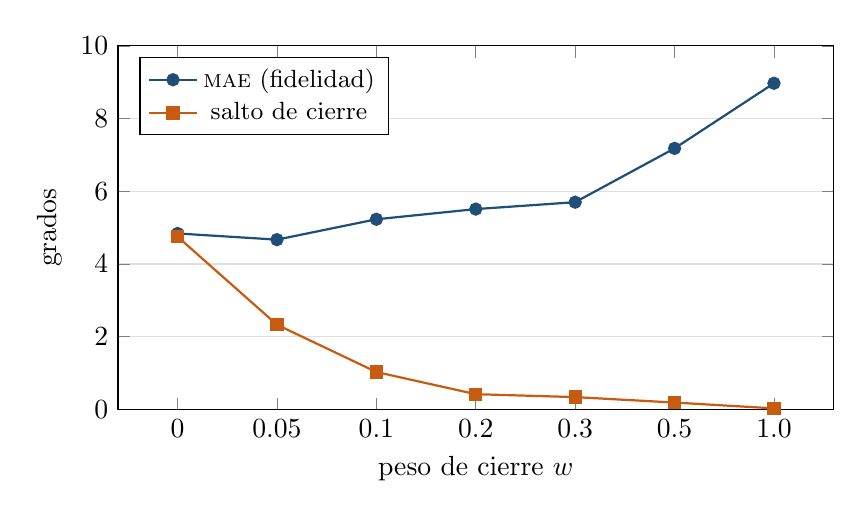
\begin{tikzpicture}
\begin{axis}[width=0.88\textwidth,height=6.2cm,xlabel={peso de cierre $w$},ylabel={grados},
 symbolic x coords={0,0.05,0.1,0.2,0.3,0.5,1.0},xtick=data,ymin=0,ymax=10,legend pos=north west,
 ymajorgrids,grid style={gray!25},legend style={font=\small}]
\addplot[color=azul,mark=*,thick] coordinates {(0,4.84)(0.05,4.67)(0.1,5.23)(0.2,5.51)(0.3,5.70)(0.5,7.18)(1.0,8.97)};
\addlegendentry{\mae{} (fidelidad)}
\addplot[color=naranja,mark=square*,thick] coordinates {(0,4.75)(0.05,2.33)(0.1,1.03)(0.2,0.42)(0.3,0.34)(0.5,0.19)(1.0,0.03)};
\addlegendentry{salto de cierre}
\end{axis}
\end{tikzpicture}
\end{center}

\begin{cuidado}[Lectura honesta de la curva]
Hay un compromiso real: el salto tiende a cero con $w$ grande, pero a costa de error. Por eso no se maximiza $w$; se elige un valor intermedio. Además, el mejor $w$ \emph{depende del tamaño del latente} (ver experimento 6).
\end{cuidado}

\subsection{Experimento 3: las dos juntas, con cinco semillas}

\begin{center}
\begin{tabular}{lcc}
\toprule
 & \textbf{\mae{} (\gr)} & \textbf{Salto (\gr)} \\
\midrule
RNN original (reproducido) & $4.99\pm0.23$ & $5.07\pm0.55$ \\
+ runa repetida + cierre ($w=0.05$) & \bpm{4.20}{0.03} & \bpm{1.33}{0.15} \\
\bottomrule
\end{tabular}
\end{center}

\begin{resultado}
La combinación gana en las cinco semillas, en ambas métricas. Además, la \emph{dispersión entre semillas cae} de $\pm0.23$ a $\pm0.03$: el modelo no solo es mejor, también es mucho más estable.
\end{resultado}

\subsection{Experimento 5: llevar lo mismo al modelo denoising}

\textbf{Qué se hizo.} Se aplicaron los mismos dos cambios al modelo denoising (el que se entrena con ciclos dañados y objetivo limpio).

\begin{center}
\begin{tabular}{lccc}
\toprule
 & \textbf{\mae{} (\gr)} & \textbf{Salto (\gr)} & \textbf{Ganancia de corrección} \\
\midrule
Denoising original (reproducido) & $5.25\pm0.10$ & $3.04\pm0.31$ & $0.296\pm0.014$ \\
Denoising + runa + cierre & \bpm{4.83}{0.07} & \bpm{0.57}{0.05} & \bpm{0.337}{0.007} \\
\midrule
Valor $p$ (prueba t pareada) & \textbf{0.0005} & $\mathbf{<0.001}$ & \textbf{0.0019} \\
\bottomrule
\end{tabular}
\end{center}

\begin{intuicion}
La mejora en corrección es modesta en términos absolutos ($0.296\to0.337$) comparada con la del salto (3.04\gr{} $\to$ 0.57\gr): su techo lo marca otra cosa, qué tan bien \emph{adivina} el modelo el ciclo limpio a partir de uno dañado. Aun así, mejoró en las cinco semillas y la diferencia es estadísticamente clara. La ganancia de tipicidad también mejoró ($0.383\to0.414$, $p=0.001$).
\end{intuicion}

\subsection{Experimento 6: un latente más grande exige re-ajustar $w$}

Al pasar el código $z$ de 16 a 32 números, la mejor pérdida de cierre cambió de $w=0.05$ a $w=0.1$ (con 32 números la red puede ``hacer trampa'' con más detalle, así que el cierre debe ser más exigente).

\begin{center}
\begin{tabular}{lcc}
\toprule
 & \textbf{\mae{} (\gr)} & \textbf{Salto (\gr)} \\
\midrule
Latente 16, $w=0.05$ & $4.20\pm0.03$ & $1.33\pm0.15$ \\
Latente 32, $w=0.1$ & \bpm{4.11}{0.05} & \bpm{0.87}{0.11} \\
\midrule
Valor $p$ & \textbf{0.018} & \textbf{0.004} \\
\bottomrule
\end{tabular}
\end{center}

\begin{intuicion}[Lección general]
Los hiperparámetros no son independientes. Si se cambia el tamaño del código, el peso de la penalización debe revisarse. Probar un latente más grande \emph{sin} re-ajustar $w$ habría dado una conclusión engañosa.
\end{intuicion}

\subsection{Experimento 7: ensamble de cinco semillas}

Promediar las predicciones de cinco modelos entrenados con semillas distintas baja el error a \textbf{3.91\gr{}} (salto 0.55\gr) para A, y a \textbf{4.74\gr{}} (salto 0.36\gr, corrección 0.349) para B. Cada cifra viene de un único ensamble, sin incertidumbre medida.

\begin{intuicion}
Cada modelo se equivoca un poco distinto por azar. Al promediar, los errores aleatorios se cancelan, como cuando se promedian varias mediciones de una misma cosa. Lo que \emph{no} se cancela es un error sistemático (algo que todos los modelos hacen mal por igual).
\end{intuicion}

%=====================================================================
\section{La sugerencia de la reunión: penalizar entre $t$ y $t-1$}
\label{sec:suavidad}

La interpretación adoptada fue: añadir una penalización por diferencias entre pasos consecutivos de la salida (suavidad), y también sobre la segunda diferencia (aceleración).

\textbf{Resultado} (una semilla, sobre la propuesta de la runa repetida):

\begin{center}
\begin{tabular}{lccc}
\toprule
Peso de suavidad & 0 & 0.2 & 3.0 \\
\midrule
\mae{} (\gr) & 4.219 & \textbf{4.215} & 4.451 \\
Salto de cierre (\gr) & 3.912 & \textbf{3.907} & 5.862 \\
\bottomrule
\end{tabular}
\end{center}

Con pesos pequeños no cambia nada (diferencias de milésimas); con pesos grandes empeora. Con la segunda diferencia (aceleración) ocurre lo mismo (\mae{} 4.219 $\to$ 4.212 con peso 1.0; salto 3.912 $\to$ 3.941). Combinadas con el cierre, tampoco aportan (\mae{} 4.182 en todos los casos).

\begin{intuicion}[{Por qué no ayuda, y qué sí captura la idea}]
Una GRU ya produce salidas suaves de forma natural, porque su estado cambia gradualmente de un paso al siguiente. Pedirle suavidad es pedirle algo que ya hace. El problema real no está \emph{dentro} del ciclo sino en la \emph{costura}: el punto 100 y el punto 0 son vecinos en el tiempo (el $t-1$ del primer punto es el último). Esa es justamente la pérdida de cierre, que sí funcionó. Dicho de otro modo: la intuición de ``mirar $t$ contra $t-1$'' era buena, pero la diferencia que importaba era la que cruza el borde del ciclo.
\end{intuicion}

\begin{cuidado}[Para confirmar con el tutor]
Esta es una \emph{lectura} de lo que se sugirió. Conviene preguntar si se refería a esto, a un término de periodicidad como el del kernel periódico del proceso gaussiano, o a una ponderación distinta entre instantes.
\end{cuidado}

\subsection{Las otras lecturas de la sugerencia}
\label{sec:otras}

Como la sugerencia admitía varias lecturas, se probaron las demás. Se exploró con una semilla y las variantes más prometedoras se validaron con cinco semillas (modelo A, latente 16, con prueba t pareada).

\begin{center}
\small
\begin{tabularx}{\textwidth}{@{}>{\raggedright\arraybackslash}p{3.1cm}>{\raggedright\arraybackslash}X>{\raggedright\arraybackslash}p{4.4cm}@{}}
\toprule
\textbf{Lectura} & \textbf{Intuición} & \textbf{Qué pasó (1 semilla)} \\
\midrule
Suavidad circular & Penalizar $|\hat G_t-\hat G_{t-1}|$ contando también el paso del punto 100 al 0. & Cierra el ciclo solo en parte (salto 3.1\gr{} frente a 3.9\gr{} sin nada, contra 1.1\gr{} con la pérdida de cierre). \\
Curvatura circular & Penalizar la segunda diferencia: evita ``esquinas'', también en la costura. & Baja la pendiente en la costura y la rugosidad; el error no cambia. \\
Igualar incrementos & Exigir que el cambio de $t-1$ a $t$ se parezca al cambio \emph{real}, no solo el valor. & Mejora levemente el error en los incrementos y la pendiente en la costura; el salto de cierre sube. \\
Pendiente en la costura & Exigir que la pendiente al final iguale la del inicio (continuidad de la derivada). & Casi elimina el quiebre (pendiente 1.38 $\to$ 0.13), con un pequeño costo en error. \\
Kernel periódico & Que puntos cercanos en fase circular tengan valores cercanos, como en el proceso gaussiano periódico. & Con peso fuerte el error sube a 4.98\gr{}; con peso suave no aporta. \\
Peso por fase & Dar más peso al error cerca de los extremos del ciclo. & El error baja (4.11\gr{}) pero el salto de cierre sube a 3.3\gr{}. \\
\bottomrule
\end{tabularx}
\end{center}

\begin{intuicion}[Qué mide cada columna nueva]
Además del error y del salto de cierre se midieron tres cosas sobre la \emph{forma} de la curva:
\textbf{pendiente en la costura} (cuánto difiere la pendiente al final y al inicio: un ``quiebre'' visible al encadenar zancadas), \textbf{error en los incrementos} (si los cambios paso a paso se parecen a los reales) y \textbf{rugosidad} (promedio de la segunda diferencia: qué tan ``dentada'' es la curva). Todas en grados; menor es mejor.
\end{intuicion}

\textbf{Validación con cinco semillas} (modelo A; media $\pm$ desviación estándar):

\begin{center}
\footnotesize
\setlength{\tabcolsep}{3.5pt}
\begin{tabular}{lccccc}
\toprule
 & \mae{} & Salto & Pend. costura & Err. increm. & Rugosidad \\
\midrule
Referencia, $w=0.05$ & \bpm{4.196}{0.025} & $1.33\pm0.15$ & $1.15\pm0.19$ & $0.578\pm0.007$ & $0.118\pm0.003$ \\
Referencia, $w=0.1$ & $4.244\pm0.031$ & \bpm{0.83}{0.07} & $1.15\pm0.16$ & $0.581\pm0.008$ & $0.118\pm0.004$ \\
Incrementos, $w=0.1$ & $4.212\pm0.032$ & $0.99\pm0.12$ & $0.70\pm0.09$ & $0.557\pm0.005$ & $0.110\pm0.002$ \\
Incrementos + curvatura, $w=0.1$ & $4.214\pm0.026$ & $0.95\pm0.10$ & $0.58\pm0.07$ & \bpm{0.553}{0.003} & $0.104\pm0.002$ \\
Incrementos + pendiente, $w=0.1$ & $4.244\pm0.056$ & $0.96\pm0.06$ & \bpm{0.19}{0.02} & \bpm{0.553}{0.006} & $0.106\pm0.001$ \\
Curvatura (peso 3), $w=0.05$ & $4.248\pm0.031$ & $0.96\pm0.09$ & $0.52\pm0.04$ & $0.567\pm0.007$ & \bpm{0.094}{0.002} \\
\midrule
Ciclos reales (referencia) & -- & 6.0 & 0.81 & -- & 0.226 \\
\bottomrule
\end{tabular}
\end{center}

{\small Negrilla: mejor valor de cada columna.}

\textbf{Lectura contra la referencia con el mismo $w=0.1$:} igualar incrementos baja el error ($p=0.008$, 5/5 semillas), la pendiente en la costura ($-39\%$), el error en los incrementos ($-4\%$) y la rugosidad ($-7\%$), todos con $p<0.01$; a cambio el salto de cierre sube de 0.83\gr{} a 0.99\gr{} ($p=0.005$). Contra la referencia con $w=0.05$ (la configuración previa) el error no cambia ($p=0.31$) y el salto baja de 1.33\gr{} a 0.99\gr{} en las 5 semillas.

\textbf{En el modelo denoising (B, $w=0.07$, cinco semillas)} el patrón se repite: la pendiente en la costura baja de $1.03\pm0.17$ a $0.58\pm0.06$ con incrementos ($p=0.002$) y a $0.42\pm0.03$ con incrementos y curvatura; el error ($4.83$) y la ganancia de corrección (\(\approx0.32\) en este experimento, con otra realización del daño) no cambian.

\begin{resultado}[Conclusión sobre las otras lecturas]
Ninguna lectura mejora de forma práctica el \textbf{error de reconstrucción}: la mejor diferencia (igualar incrementos frente a la referencia con el mismo $w$) es de 0.03\gr, detectable estadísticamente pero sin importancia práctica. Dos sí mejoran la \textbf{calidad de la forma}: igualar incrementos y la curvatura circular dejan la curva menos quebrada en la costura y con cambios más parecidos a los reales, sin costo en error y a cambio de un salto de cierre algo mayor ($0.83\to0.95$--$0.99$\gr). El kernel periódico y el peso por fase no ayudan.
\end{resultado}

\begin{cuidado}[Hallazgo: los ciclos reales no cierran]
Los ciclos reales de control tienen un salto medio entre el punto 0\% y el 100\% de unos \textbf{6\gr}, y una diferencia de pendiente en la costura de 0.81\gr{} por paso. Es decir, cerrar el ciclo es un \emph{supuesto de periodicidad}, no fidelidad a los datos (el ruido de la estimación por video impide cerrar). Por eso exigir más suavidad o cierre no reduce el error, y por eso los modelos ya quedan más suaves que los datos (rugosidad 0.09--0.12 frente a 0.23 real). La penalización aporta una curva \emph{más coherente con un ciclo periódico}, no una reconstrucción más cercana a la medición.
\end{cuidado}

%=====================================================================
\section{Lo que no funcionó (y qué enseña)}
\label{sec:nofunciono}

\begin{tabularx}{\textwidth}{@{}>{\raggedright\arraybackslash}p{3.3cm}>{\raggedright\arraybackslash}X>{\raggedright\arraybackslash}p{4.5cm}@{}}
\toprule
\textbf{Experimento} & \textbf{Qué se probó y qué pasó} & \textbf{Por qué probablemente} \\
\midrule
Decodificador bidireccional & Con la misma configuración, \mae{} 4.244 / salto 3.920 (sin cierre) y 4.273 / 1.072 (con cierre), frente a 4.219 / 3.912 y 4.182 / 1.140 con el unidireccional. No mejora. & El decodificador ya recibe $z$ y la fase en cada paso; mirar ``hacia atrás'' no agrega información útil. \\
Atención en el codificador & El \mae{} subió a $\approx8.5$\gr{} y los pesos de atención quedaron casi uniformes ($\approx 0.011$ cada uno, es decir $1/101$). Con temperatura muy baja, 5.6\gr. & Con 240 ciclos no hay datos suficientes para aprender \emph{dónde mirar}; la atención degenera en un promedio. \\
Velocidad angular como entrada extra (B) & \mae{} 4.728 $\to$ 4.822 (peor). & La derivada amplifica el ruido de los ángulos estimados por video. \\
Asimetría izquierda-derecha (B) & \mae{} 4.728 $\to$ 4.771; corrección 0.349 $\to$ 0.333. & La información ya está en los seis canales; el extra solo agrega parámetros. \\
Consistencia del latente (B) & Peso 0.05: \mae{} 4.833 vs 4.835, corrección 0.320 vs 0.322 ($p=0.85$ y $0.40$). Con 0.5, empeora (4.935). & El denoising ya induce códigos parecidos; forzarlo más no suma. \\
Intensidad de corrupción & 0.5: \mae{} 4.45, corrección 0.320; 1.0: 4.73 / 0.349; 1.5: 5.12 / 0.329. & La corrección alcanza su máximo con la intensidad 1.0 (U invertida; el \mae{} sube siempre porque la tarea se hace más difícil): la receta original ya estaba bien calibrada. \\
Currículo de corrupción (de 0.2 a 1.0) & \mae{} $4.83\to4.79$, corrección $0.320\to0.324$ ($p=0.26$ y $0.51$). & Efecto dentro del ruido entre semillas. \\
Ensamble mixto A + B & \mae{} 4.160, corrección 0.319: queda \emph{entre} los dos. & Ver sección \ref{sec:ab}: los dos modelos tienen objetivos distintos. \\
\bottomrule
\end{tabularx}

\begin{intuicion}[Qué enseñan en conjunto los fracasos]
Casi todos los intentos de ``agregarle algo'' al modelo no sirvieron. Eso indica que el cuello de botella ya no es la arquitectura sino el \textbf{tamaño de los datos} (240 ciclos de entrenamiento, 28 personas). Con tan pocos datos, añadir componentes aprendibles (atención, más entradas) añade más ruido que señal.
\end{intuicion}

%=====================================================================
\section{Dos modelos, dos trabajos: A y B}
\label{sec:ab}

\begin{tabularx}{\textwidth}{@{}>{\bfseries}p{3.0cm}XX@{}}
\toprule
 & \textbf{A} (\texttt{rnn\_autoencoder}) & \textbf{B} (\texttt{denoising\_rnn\_autoencoder}) \\
\midrule
Se entrena con & Ciclos limpios $\to$ los mismos ciclos & Ciclos \emph{dañados} $\to$ ciclos limpios \\
Pregunta que responde & ¿Qué tan fielmente puedo reconstruir? & Si llega un ciclo raro, ¿cómo sería la versión típica? \\
Fortaleza & Mejor \mae{} de las dos (\textbf{3.91\gr{}} en ensamble) & Mejor corrección de las dos (\textbf{0.349} en ensamble) \\
Riesgo & Reproduce también lo anómalo & Se aleja un poco de la entrada \\
\bottomrule
\end{tabularx}

\begin{intuicion}[Analogía]
A es una fotocopiadora de alta calidad: copia lo que le muestran, defectos incluidos. B es un restaurador: recibe una pintura estropeada y devuelve cómo \emph{debería} verse. Si se mezclan en un solo ensamble, se obtiene una fotocopiadora que a veces restaura: queda en un punto intermedio (\mae{} 4.16\gr, corrección 0.319), sin superar a cada uno en lo suyo.
\end{intuicion}

\begin{cuidado}[Un matiz sobre A]
En el cuaderno original, A tenía una ganancia de tipicidad alta (0.349, cercana a la de B, 0.385). Esto no contradice la analogía: A también tenía una de las mayores intervenciones (8.12\gr, por su error de reconstrucción alto), es decir, su salida se aleja de la entrada sin que eso sea una corrección deliberada. Con cinco semillas, el A reproducido tiene tipicidad $0.345\pm0.008$ y el A mejorado $0.326\pm0.007$ ($p=0.034$, sin corrección por multiplicidad; $0.358$ en ensamble), y su intervención baja de 7.78\gr{} a 6.14\gr: el modelo mejorado copia con más fidelidad y se aleja menos de la entrada. Por qué baja la tipicidad no se probó.
\end{cuidado}

\textbf{¿Y por qué no usar PCA, que tiene \mae{} 2.78\gr?} Porque PCA es excelente \emph{reproduciendo}, pero precisamente por eso reproduce también lo atípico: su ganancia de tipicidad es la más baja de todos los modelos (0.127, frente a 0.349 y 0.385 de los RNN originales). Para el objetivo de corregir trayectorias hacia lo típico, la fidelidad pura no es lo que se busca. Para el objetivo de fidelidad pura, PCA sigue ganando; el RNN todavía no la alcanza. Además, aunque B mejoró, su ganancia de corrección (0.337 con un modelo, 0.349 con ensamble) sigue por debajo de la del autoencoder convolucional denoising del cuaderno original (0.412): mejorar la RNN no la convierte en la mejor opción para corregir; es una pregunta abierta si conviene aplicar los mismos cambios a ese modelo.

%=====================================================================
\section{La escalera de mejora}
\label{sec:escalera}

\newcommand{\barchart}[2]{%
\begin{tikzpicture}[x=#2,y=-0.62cm]
 \foreach \lab/\val/\cls [count=\i from 0] in {#1}{
  \ifnum\cls=1 \def\col{azul}\else\def\col{gris!55}\fi
  \node[anchor=east,font=\small] at (-0.15,\i) {\lab};
  \fill[\col] (0,\i-0.3) rectangle (\val,\i+0.3);
  \node[anchor=west,font=\scriptsize] at (\val+0.05,\i) {\val};
 }
 \draw[gray] (0,-0.6) -- (0,9.6);
\end{tikzpicture}}

\textbf{Error de reconstrucción (\mae{}, grados; menor es mejor)}

\begin{center}
\barchart{RNN original (cuaderno)/5.17/0, RNN original (reproducido)/4.99/0, A: runa y cierre/4.20/1, A: latente 32/4.11/1, A: ensamble de 5/3.91/1, Denoising original (cuaderno)/5.35/0, B: runa y cierre/4.83/1, B: ensamble de 5/4.74/1, Proceso gaussiano periódico/3.30/0, PCA/2.78/0}{1.35cm}
\end{center}

\textbf{Salto de cierre (grados; menor es mejor)}

\begin{center}
\barchart{RNN original (cuaderno)/4.94/0, RNN original (reproducido)/5.07/0, A: runa y cierre/1.33/1, A: latente 32/0.87/1, A: ensamble de 5/0.55/1, Denoising original (cuaderno)/3.45/0, B: runa y cierre/0.57/1, B: ensamble de 5/0.36/1, Proceso gaussiano periódico/0.60/0, PCA/3.41/0}{1.35cm}
\end{center}
{\small Gris: referencias (cuaderno original, reproducción propia, otros modelos). Azul: versiones mejoradas. Barras de 1 modelo = promedio de 5 semillas; ``ensamble'' = un ensamble de 5.}

\subsection*{Cuánto se mejoró, en porcentajes}

\begin{center}
\small
\begin{tabular}{lccc}
\toprule
 & \textbf{Original} & \textbf{Mejorado, 1 modelo} & \textbf{Mejorado, ensamble de 5} \\
\midrule
Modelo A: \mae{} (\gr) & 5.17 & 4.11 ($-20\%$) & \textbf{3.91} ($-24\%$) \\
Modelo A: salto (\gr) & 4.94 & 0.87 ($-82\%$) & \textbf{0.55} ($-89\%$) \\[3pt]
Modelo B: \mae{} (\gr) & 5.35 & 4.83 ($-10\%$) & \textbf{4.74} ($-11\%$) \\
Modelo B: salto (\gr) & 3.45 & 0.57 ($-84\%$) & \textbf{0.36} ($-90\%$) \\
Modelo B: ganancia de corrección & 0.280 & 0.337 ($+20\%$) & \textbf{0.349} ($+25\%$) \\
\bottomrule
\end{tabular}
\end{center}

\textbf{Cómo leer las dos columnas ``mejorado''.} ``1 modelo'' es el promedio de 5 modelos entrenados por separado (uno por semilla); es la cifra \emph{validada} con prueba t. ``Ensamble de 5'' promedia las \emph{predicciones} de esos 5 modelos: es mejor en todas las métricas, pero cuesta cinco modelos y proviene de un único ensamble, sin incertidumbre medida. Para A, ``mejorado'' incluye además latente de 32 y $w=0.1$; para B, latente de 16.

\begin{cuidado}[Dos comparaciones posibles]
Estos porcentajes comparan contra los números que figuran en el cuaderno original. Contra la reproducción propia del modelo original (4.99 y 5.25 de \mae{}) las mejoras son algo menores en fidelidad: $-18\%$ para A y $-8\%$ para B. Ambas comparaciones son legítimas; la segunda es la más estricta porque usa exactamente el mismo protocolo.
\end{cuidado}

%=====================================================================
\section{Limitaciones y salvedades honestas}
\label{sec:limites}

\begin{enumerate}
\item \textbf{Los hiperparámetros se eligieron mirando \emph{control\_test}.} Es el mismo conjunto en el que se reportan los resultados, así que las cifras finales son algo optimistas. Lo correcto sería elegir con validación o con validación cruzada por sujeto, y reservar el test para el final.
\item \textbf{Latentes 32/48/64 en el modelo B no están distinguidos.} Con 5 semillas, el paso de 16 a 32 en B dio \mae{} $4.83\to4.77$ ($p=0.52$) y corrección $0.32\to0.33$ ($p=0.18$): no es significativo. Los ensambles de 32, 48 y 64 (4.68, 4.67, 4.55 de \mae{}) son un solo ensamble cada uno y no se midió cuánto varía un ensamble de otro, así que no se sabe si esas diferencias (hasta 0.19\gr) son reales. No debe afirmarse que ``64 es el mejor''.
\item \textbf{Un solo ensamble por configuración.} Los números de ensamble vienen de un único conjunto de 5 modelos; su incertidumbre no se midió.
\item \textbf{Una sola perturbación para la evaluación II.} La ganancia de corrección se calcula con una realización del daño aleatorio. La corrección de B mejorado fue $0.32\pm0.02$ en los experimentos en que cada semilla usó una realización distinta del daño y $0.337\pm0.007$ con la realización fija usada en esta versión de la guía: una variabilidad del orden de 0.02 atribuible a la evaluación. Dentro de cada experimento las dos ramas comparadas usan la misma realización, pero las cifras absolutas de experimentos distintos (por ejemplo, la tabla de latentes y la de intensidad del daño) no son directamente comparables entre sí.
\item \textbf{Comparación del decodificador bidireccional.} La referencia unidireccional venía de otro estado de azar; la comparación justa es la de la tabla de la sección \ref{sec:nofunciono} (misma configuración), donde tampoco mejora.
\item \textbf{Los datos fueron reconstruidos} a partir de los archivos entregados. Las cifras originales del cuaderno (5.17 y 5.35) y las reproducidas (4.99 y 5.25) difieren ligeramente; conviene correr el cuaderno original del tutor en la máquina propia para confirmar.
\item \textbf{El autoencoder convolucional denoising} del cuaderno original (corrección 0.412) no fue mejorado ni reevaluado con el protocolo de cinco semillas; la comparación con B mejorado es indicativa.
\item \textbf{Las otras lecturas de $t$ y $t-1$} se validaron solo en el modelo A (y las dos más prometedoras en B); la exploración amplia usó una semilla, y la elección de pesos se hizo sobre el conjunto de prueba de control.
\item \textbf{Los guiones de los experimentos viven en el entorno de trabajo}; el cuaderno entregado (13) incluye solo la runa repetida y el cierre. Los guiones de todos los experimentos fueron entregados aparte (archivo comprimido de experimentos).
\end{enumerate}

%=====================================================================
\section{Guion para la reunión}

\subsection{Relato en cinco pasos (unos cinco minutos)}

\begin{enumerate}
\item \textbf{Diagnóstico.} ``El RNN era el peor modelo. Encontré dos causas: el decodificador olvidaba el código, y nada pedía que el ciclo cerrara.''
\item \textbf{Dos cambios.} ``Repetí el código en cada paso y añadí una penalización de cierre. Con cinco semillas, el error bajó de 5.0 a 4.2 y el salto de 5.0 a 1.3, con una variabilidad mucho menor.''
\item \textbf{Extensión.} ``Lo mismo mejora el denoising: salto de 3.0 a 0.57 y corrección de 0.30 a 0.34, significativo. Con un latente de 32 y $w=0.1$ el modelo simple llega a 4.11 y 0.87; el ensamble, a 3.91 y 0.55.''
\item \textbf{Lo que no sirvió.} ``Probé suavidad, atención, características extra, consistencia, currículo y decodificador bidireccional. Ninguno ayuda, y eso apunta a que el límite está en la cantidad de datos.''
\item \textbf{Hacia dónde ir.} ``A y B hacen trabajos distintos. Propongo validación cruzada por sujeto y definir qué error es suficiente para la aplicación.''
\end{enumerate}

\subsection{Preguntas probables y respuestas cortas}

\begin{tabularx}{\textwidth}{@{}>{\raggedright\arraybackslash}p{5.2cm}X@{}}
\toprule
\textbf{Pregunta} & \textbf{Respuesta} \\
\midrule
¿Por qué no usar PCA si tiene menos error? & PCA reconstruye muy bien, pero reproduce también lo atípico (tipicidad 0.127). Para corregir trayectorias, B supera a PCA (0.349 frente a 0.207); para fidelidad pura, PCA gana. \\
¿Cómo sé que no es suerte de la semilla? & Cinco semillas y prueba t pareada: las mejoras de la sección \ref{sec:mejoras} ganan en 5/5 semillas; en los contrastes pareados calculados (denoising, latente 32), $p<0.02$. \\
¿Por qué el cierre cuesta algo de error? & Es un compromiso: cuanto más se fuerza el cierre, menos libertad tiene la curva. Se escogió un $w$ pequeño donde el salto cae mucho y el error casi no sube. \\
¿Por qué no probar atención, que es más moderna? & Se probó y colapsó a un promedio uniforme: con 240 ciclos no aprende dónde mirar. \\
¿Cuál es el mejor modelo? & Ninguno gana en todo (sección \ref{sec:veredicto}). Para reconstruir, A en ensamble: \mae{} 3.91\gr{} (original 5.17\gr, $-24\%$) y salto 0.55\gr. Para corregir, B en ensamble: corrección 0.349 (original 0.280, $+25\%$). El autoencoder convolucional denoising del cuaderno original (0.412) sigue por encima en corrección, y PCA (2.78\gr) en \mae{}. Entre las variantes de latente de B no hay diferencia estadística. \\
¿Se probaron otras lecturas de $t$ y $t-1$? & Sí: suavidad y curvatura circular, igualar incrementos, pendiente en la costura, kernel periódico y peso por fase. No bajan el error; igualar incrementos y la curvatura mejoran la forma en la costura (sección \ref{sec:otras}). \\
Entonces, ¿por qué no usar PCA ni el convolucional denoising? & Con las cifras actuales no hay razón basada en métricas: PCA gana en \mae{} (2.78\gr) y el convolucional denoising en corrección (0.412). La RNN solo queda al frente en cierre de ciclo. Se propone aplicar las mejoras al convolucional y reevaluar todo con cinco semillas (sección \ref{sec:veredicto}). \\
¿Cuánto error es suficiente? & Es justo la pregunta que conviene hacerle al tutor: depende de la tolerancia clínica y de qué tan lejos queda una trayectoria atípica de una típica. \\
\bottomrule
\end{tabularx}

\subsection{Preguntas para el tutor}
\begin{itemize}
\item De las lecturas probadas de $t$ y $t-1$ (sección \ref{sec:otras}), ¿cuál se acerca más a lo que se tenía en mente? ¿Interesa más la forma de la curva (continuidad) o el error de reconstrucción?
\item ¿Qué error de reconstrucción o de corrección se considera suficiente para la aplicación con el exoesqueleto?
\item ¿Se prefiere priorizar fidelidad (A) o corrección (B) como modelo de referencia del proyecto?
\item ¿Se mejora la RNN por decisión de diseño, o se busca el mejor modelo? Con las cifras actuales, PCA gana en fidelidad y el convolucional denoising en corrección.
\item ¿Se aceptaría validación cruzada por sujeto para elegir hiperparámetros, dado el tamaño de los datos?
\end{itemize}

\subsection{Próximos pasos propuestos}
\begin{enumerate}
\item Aplicar al autoencoder convolucional denoising las mejoras que funcionaron y reevaluarlo, junto con PCA, con cinco semillas y el mismo protocolo (sección \ref{sec:veredicto}).
\item Validación cruzada por sujeto (elegir con validación, reportar en test una sola vez).
\item Repetir los ensambles varias veces para medir su incertidumbre y decidir de verdad entre latentes 32/48/64 en B.
\item Evaluar los modelos finales en la evaluación III (casos externos).
\item Más datos o aumento de datos realista: es el cuello de botella que sugieren los experimentos negativos.
\item Empaquetar los experimentos adicionales en el cuaderno.
\end{enumerate}

%=====================================================================
\appendix
\section{Apéndice: resultados por semilla}

\small
\textbf{Modelo A: latente 16 con $w=0.05$ frente a latente 32 con $w=0.1$.}
\begin{center}
\begin{tabular}{rcccc}
\toprule
 & \multicolumn{2}{c}{\mae{} (\gr)} & \multicolumn{2}{c}{Salto (\gr)} \\
\cmidrule(lr){2-3}\cmidrule(lr){4-5}
Semilla & 16 & 32 & 16 & 32 \\
\midrule
42 & 4.182 & 4.038 & 1.140 & 0.968 \\
1 & 4.208 & 4.163 & 1.494 & 0.985 \\
7 & 4.234 & 4.118 & 1.198 & 0.771 \\
123 & 4.178 & 4.147 & 1.358 & 0.759 \\
2024 & 4.176 & 4.099 & 1.433 & 0.843 \\
\midrule
Media $\pm$ d.e. & $4.196\pm0.025$ & \bpm{4.113}{0.049} & $1.325\pm0.151$ & \bpm{0.865}{0.107} \\
\bottomrule
\end{tabular}
\end{center}

\textbf{Modelo B: original frente a runa + cierre (latente 16, $w=0.05$).}
\begin{center}
\begin{tabular}{rcccccc}
\toprule
 & \multicolumn{2}{c}{\mae{}} & \multicolumn{2}{c}{Salto} & \multicolumn{2}{c}{Corrección} \\
\cmidrule(lr){2-3}\cmidrule(lr){4-5}\cmidrule(lr){6-7}
Semilla & orig. & mejor. & orig. & mejor. & orig. & mejor. \\
\midrule
42 & 5.250 & 4.739 & 3.194 & 0.590 & 0.298 & 0.348 \\
1 & 5.328 & 4.839 & 3.418 & 0.598 & 0.281 & 0.332 \\
7 & 5.358 & 4.938 & 3.040 & 0.525 & 0.283 & 0.333 \\
123 & 5.171 & 4.786 & 2.998 & 0.512 & 0.304 & 0.333 \\
2024 & 5.120 & 4.831 & 2.569 & 0.611 & 0.313 & 0.339 \\
\midrule
Media & 5.245 & \textbf{4.827} & 3.044 & \textbf{0.567} & 0.296 & \textbf{0.337} \\
\bottomrule
\end{tabular}
\end{center}

\textbf{Modelo B: ajuste del peso de cierre (latente 16, una semilla).}
\begin{center}
\begin{tabular}{lcccccc}
\toprule
$w$ & 0.02 & 0.03 & 0.05 & 0.07 & 0.10 & 0.15 \\
\midrule
\mae{} & 4.731 & 4.729 & 4.741 & \textbf{4.728} & 4.753 & 4.787 \\
Salto & 1.002 & 0.693 & 0.585 & 0.460 & 0.624 & \textbf{0.324} \\
Corrección & 0.347 & \textbf{0.349} & 0.348 & \textbf{0.349} & 0.346 & 0.343 \\
\bottomrule
\end{tabular}
\end{center}
Con cinco semillas, pasar de $w=0.05$ a $0.07$ baja el salto de $0.57\pm0.05$ a $0.47\pm0.09$ ($p=0.022$, 4 de 5 semillas), sin cambio en \mae{} ($p=0.57$).

\textbf{Ensambles de 5 modelos (B), evaluación I y II.}
\begin{center}
\begin{tabular}{lccc}
\toprule
Configuración & \mae{} & Salto & Corrección \\
\midrule
Latente 16, $w=0.05$ & 4.743 & 0.361 & 0.349 \\
Latente 16, $w=0.07$ & 4.746 & 0.290 & 0.349 \\
Latente 32, $w=0.1$ & 4.682 & 0.286 & 0.357 \\
Latente 48, $w=0.1$ & 4.670 & \textbf{0.248} & 0.359 \\
Latente 64, $w=0.1$ & \textbf{4.554} & 0.304 & \textbf{0.369} \\
\bottomrule
\end{tabular}
\end{center}
Un solo ensamble por fila; no se midió cuánto varía un ensamble de otro, por lo que no se sabe si las diferencias entre filas son reales (sección \ref{sec:limites}). Negrilla: mejor valor de cada columna; la cifra principal del documento es la de la primera fila.

\textbf{Modelo A en ensamble:} \mae{} \textbf{3.907}, salto \textbf{0.550}, corrección 0.229. \textbf{Mezcla A + B (10 modelos):} \mae{} 4.160, salto 0.392, corrección 0.319.

\end{document}
